\documentclass[reprint, english, nofootinbib]{revtex4-2}

\usepackage{graphicx}
\usepackage{subfig}
\usepackage[colorlinks=true,urlcolor=blue,citecolor=blue]{hyperref}
\usepackage{physics}
\usepackage{amsmath}
\usepackage{amssymb}
\usepackage{amsbsy}
\usepackage{subfig}
\usepackage{blindtext}
\usepackage{tikzducks}
\usepackage{tikz}
\usepackage{pgfplots}
\usepackage{listings}

\graphicspath{{../figs/}}


\begin{document}
\title{Solving partial differential equations with neural networks}
\author{Nicholas Karlsen}
\affiliation{University of Oslo}
\author{Thore Espedal Moe}
\affiliation{University of Oslo}
\date{\today}

\begin{abstract}
    An abstract abstract
\end{abstract}

\maketitle


\section{Introduction}

\section{Theory}
\subsection{The Heat Equation}
\noindent 
In physics, the Heat equation models how the temperature of some material $u\qty(\pmb r, t)$ evolves over time by the partial differential equation (PDE)
\begin{equation}
    \pdv{u}{t} = c^2\nabla^2 u 
\end{equation}
where $c^2$, the thermal diffusivity is a material dependent constant. 
This may be reduced to a one dimensional problem, modelling i.e a thin, insulating wire of length $L$ as
\begin{equation}\label{eqn: 1D heat eqn}
    \pdv{u}{t} = \pdv[2]{u}{t}
\end{equation}
where we have also for simplicity set $c^2 = 1$. We may then solve this analytically with boundary conditions $u\qty(0, t) = u\qty(L,t) = 0$ and initial condition $u(x, 0) = f(x)$.

We start by making the assumption that $u(x, t)$ is separable, giving 
\begin{equation}
    u(x, t) = F(x) \cdot G(t)
\end{equation}
which lets us rewrite Eqn.~\ref{eqn: 1D heat eqn} to the form
\begin{equation}
    F \cdot \pdv{G}{t} = \pdv[2]{F}{x} \cdot G
\end{equation}
which may be expressed as
\begin{equation}
    \frac{\dot G}{G} = \frac{F^{''}}{F} = k
\end{equation}
where $k$ is some constant. We further have that the boundary conditions may only be satisfied for $k <  0$, so we set $k = -\rho^2$ and write
\begin{equation}
    F^{''} + \rho F = 0 \quad \quad \dot G + \rho^2G = 0
\end{equation}
starting with the spatial equation, we have a general solution in the form 
\begin{equation}
    F(x) = c_1 \cos(\rho x) + c_2 \sin(\rho x)
\end{equation}
where $c_1 = 0$ is fixed by $u(0, t) = $. Similarly, $u(L, t) = 0$ imposes the requirement $\sin(\rho x) = 0$ which is satisfied by setting $\rho = n\pi/L$, yielding a discrete spectrum of solutions
\begin{equation}
    F_n(x) = \sin\qty(\frac{n\pi x}{L})
\end{equation}
where we omit the constant $c_1$, which we will include later in $G(t)$. 

We then move on to the temporal part, $G(t)$, which we write as
\begin{equation}
    \dot G = -\rho^2G
\end{equation}
which we immediately recognize as having a general solution
\begin{equation}
    G(t) = c_n e^{-n\pi t / L}
\end{equation}
Thus, $u(x, t)$ is solved by a superposition of the discrete set of eigenfunctions
\begin{equation}
    u_n\qty(x, t) = \sum_{n=1}^{\infty} c_n \sin\qty(\frac{n\pi x}{L}) e^{-n\pi t / L}
\end{equation}
with initial condition
\begin{equation}
    u(x, 0) = \sum_{n=1}^{\infty} c_n \sin\qty(\frac{n\pi x}{L}) = f(x)
\end{equation}
a Fourier series. Thus, the coefficients $c_n$ are determined by the integral
\begin{equation}
    c_n = \frac{2}{L}\int_0^L \dd x \, f(x) \sin\qty(\frac{n\pi x}{L})
\end{equation}
if we set the initial condition $f(x) = \sin(\pi x)$ and fix $L = 1$, we get coefficients
\begin{equation}
    c_n = 2\int_0^1 \dd x \, \sin(\pi x) \sin(n\pi x) = 1
\end{equation}
we thus have an analytical solution for the Heat equation with boundary conditions $u(0, t) = u(L, t) = 0$, $L = 1$, and initial condition $u(x, 0) = \sin(\pi x)$ as
\begin{equation}
    u(x, t) = \sin\qty(\pi x) e^{-\pi t}
\end{equation}
a plot of which for $t \in [0, 1]$ is shown in Fig.~\ref{fig: heat eqn analytic}.
\begin{figure}[h!tb]
    \center
    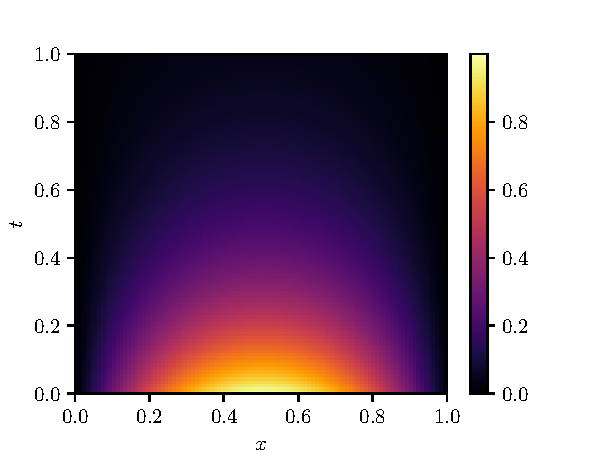
\includegraphics[width=.8\columnwidth]{heat_eqn_analytic.pdf}
    \caption{\label{fig: heat eqn analytic}}
\end{figure}

\section{Results \& Discussion}

\section{Conclusion}

\onecolumngrid
\bibliography{bibfile}
\twocolumngrid

\end{document}